\documentclass{aa}
\usepackage[varg]{txfonts}
\usepackage{graphicx}
\usepackage{color}
\usepackage{hyperref}


\usepackage{natbib}
\bibpunct{(}{)}{;}{a}{}{,} % to follow the A&A style

\newcommand{\comment}[1]{{\textcolor[rgb]{1, 0, 0}{[{\bf Comment}: #1]}}}


\begin{document}



\title{The Large Scale Polarization Explorer (LSPE) for CMB measurements: performance forecast}
\author{The LSPE collaboration}
\date{}

\abstract{Context: }
{We present the updated performance forecast of the Large Scale Polarization Explorer (LSPE),
a program dedicated to the measurement of the polarization of the cosmic microwave
background radiation (CMB). LSPE is composed of two instruments: LSPE-STRIP 
(Survey TeneRIfe Polarimeter), a radiometer based telescope on the ground in Tenerife; 
the LSPE-SWIPE (Short-Wavelength Instrument for 
the Polarization Explorer) a bolometer based instrument to fly on a winter arctic stratospheric 
long duration balloon.}
{Methods}
{Results}
{The LSPE can reach a sensitivity in tensor-to-scalar ratio of $\sigma_r<0.013$.} 


\keywords{
Instrumentation: polarimeters;
Cosmology: observations;
Cosmology: early Universe
}

\maketitle

\tableofcontents

\section{Introduction}

\comment{From LSPE program requirement; add references}\\
The Large Scale Polarization explorer (LSPE) is designed to measure the polarization of the 
Cosmic Microwave Background (CMB) at large
angular scales, and in particular to constrain the curl component of CMB polarization (B-modes).
This is produced by tensor perturbations generated during cosmic inflation, in the very early Universe.
The level of this signal is unknown: current inflation models are unable to provide a reference
value. However, the detection of this signal would be of utmost importance, providing a way to
measure the energy-scale of inflation and a window on the physics at extremely high energies.
While the level of CMB anisotropy is of the order of $100\,\mu$K rms and the level of the gradient
component of CMB polarization (E-modes generated by scalar - density perturbations) is of the order
of $3\,\mu$K, the current upper limits for the level of B-modes polarization are a fraction of $\mu$K,
corresponding to a ratio between the amplitude of tensor perturbations and the amplitude of scalar
perturbations $r < 0.07$ (68\% CL, see~\citet{bicep2018}). 
The target of LSPE is to improve this limit.

Additional targets of the mission are 
an improved measure of the optical depth to the 
cosmic microwave background $\tau$, measured from the large scale
E-mode CMB polarization; investigation of the so called
{\em low-$\ell$ anomaly}, a series of anomalies observed in the
large angular scales of the CMB polarization, including
lack of power, asymmetries and alignment of multipole moments \citep{planckIandS2016}
\comment{Gruppuso?}; 
wide maps of foreground polarization produced in our galaxy
by synchrotron emission and interstellar dust emission, whick will be important to map the magnetic
field in our Galaxy and to study the properties of the ionized gas and of the diffuse interstellar dust
in the Milky Way.

We set the target for the LSPE program a measurement of B-modes of CMB polarization
at a level corresponding to a tensor to scalar ratio r=0.03 with 99.7\% confidence (r=0.013 at 68\% CL)
\comment{rivedere}.
Since the expected B-mode signal in this case is smaller than the polarized foreground from our
Galaxy, a wide frequency coverage is needed to monitor precisely the foregrounds at frequencies
where they are most important, and subtract them to estimate the cosmological part of the detected
B-mode signal. For the synchrotron foreground, prominent at frequencies lower than the peak
frequency of the CMB (160 GHz), where atmospheric transmission and noise are favorable, a ground
based instrument is the most effective way to go. For the interstellar dust foreground, prominent at
frequencies higher than 160GHz, where atmospheric transmission and noise are poor, a stratospheric
balloon mission is required. For this reason (as described in greater detail below), the LSPE program
is composed of two experiments: a ground-based experiment, running the STRIP instrument
observing at 44 GHz, and a balloon-borne mission, flying the SWIPE instrument observing at 140,
220, 240 GHz.

In section~\ref{sec:instruments} we describe the two instruments with some detail. 
In section~\ref{sec:methods} we present the methods used to forecast the experiment
performance. 
In section~\ref{sec:results} we report the expected results. 
In section~\ref{sec:systematics} we describe the major systematic effects, and their 
mitigation techniques. 
Finally, in section~\ref{sec:conclusion} we draw conclusions. 



\section{The instruments}\label{sec:instruments}
The LSPE is composed by two separated instrument. 
\\ \comment{Add a table with STRIP+SWIPE basic instrumental parameters: bands, bandwidths, 
resolution, sensitivity, integration time, number of detectors, ....}

\subsection{LSPE-STRIP}
\comment{Mennella/Bersanelli: Take from STRIP design analysis report}

Instrument design:

\subsubsection{Site}


\subsubsection{Polarimeters}

\subsubsection{...}
\comment{Altro da STRIP}


\subsection{LSPE-SWIPE}
LSPE-SWIPE (Short-Wavelength Instrument for the Polarization Explorer) 
is a mm-wave polarimeter aboard of a 
stratospheric balloon, aimed at measuring the polarization 
of the Cosmic Microwave Background at large angular scales. 
The general idea of SWIPE is to maximize the sensitivity to CMB 
polarization at large scales using a very wide focal plane populated 
with multi-moded bolometers. The spectral coverage of SWIPE has 
been optimized to be very sensitive to CMB polarization with one 
wide-band channel matching the peak of CMB brightness (140 GHz, 
33\% band), and to be able to monitor and separate the signals from 
interstellar dust (the main polarized foreground at this frequency) 
monitoring it with two ancillary channels at 220 and 240 GHz. These 
are narrow-band, (5\%) to measure the slope of the specific brightness 
of Interstellar dust. 
The focal planes of SWIPE are so large that 8800 modes of the 
incoming radiation are collected, thus boosting the sensitivity of the 
polarimeter to unprecedented levels. The detectors arrays are cooled 
at 0.3K by a large cryostat, which also cools the polarization modulator 
and the entire telescope. The cryostat is mounted in a frame (the gondola) 
providing also accommodation for an attitude control system, the 
instrument power system and electronics. The gondola interfaces 
to the flight train of the stratospheric balloon through an azimuth pivot 
allowing for azimuth scans and/or spin. 
A general view of the SWIPE instrument is shown in Figure~\ref{fig:swipe_overview}.
   \begin{figure}[h!]
   \centering
   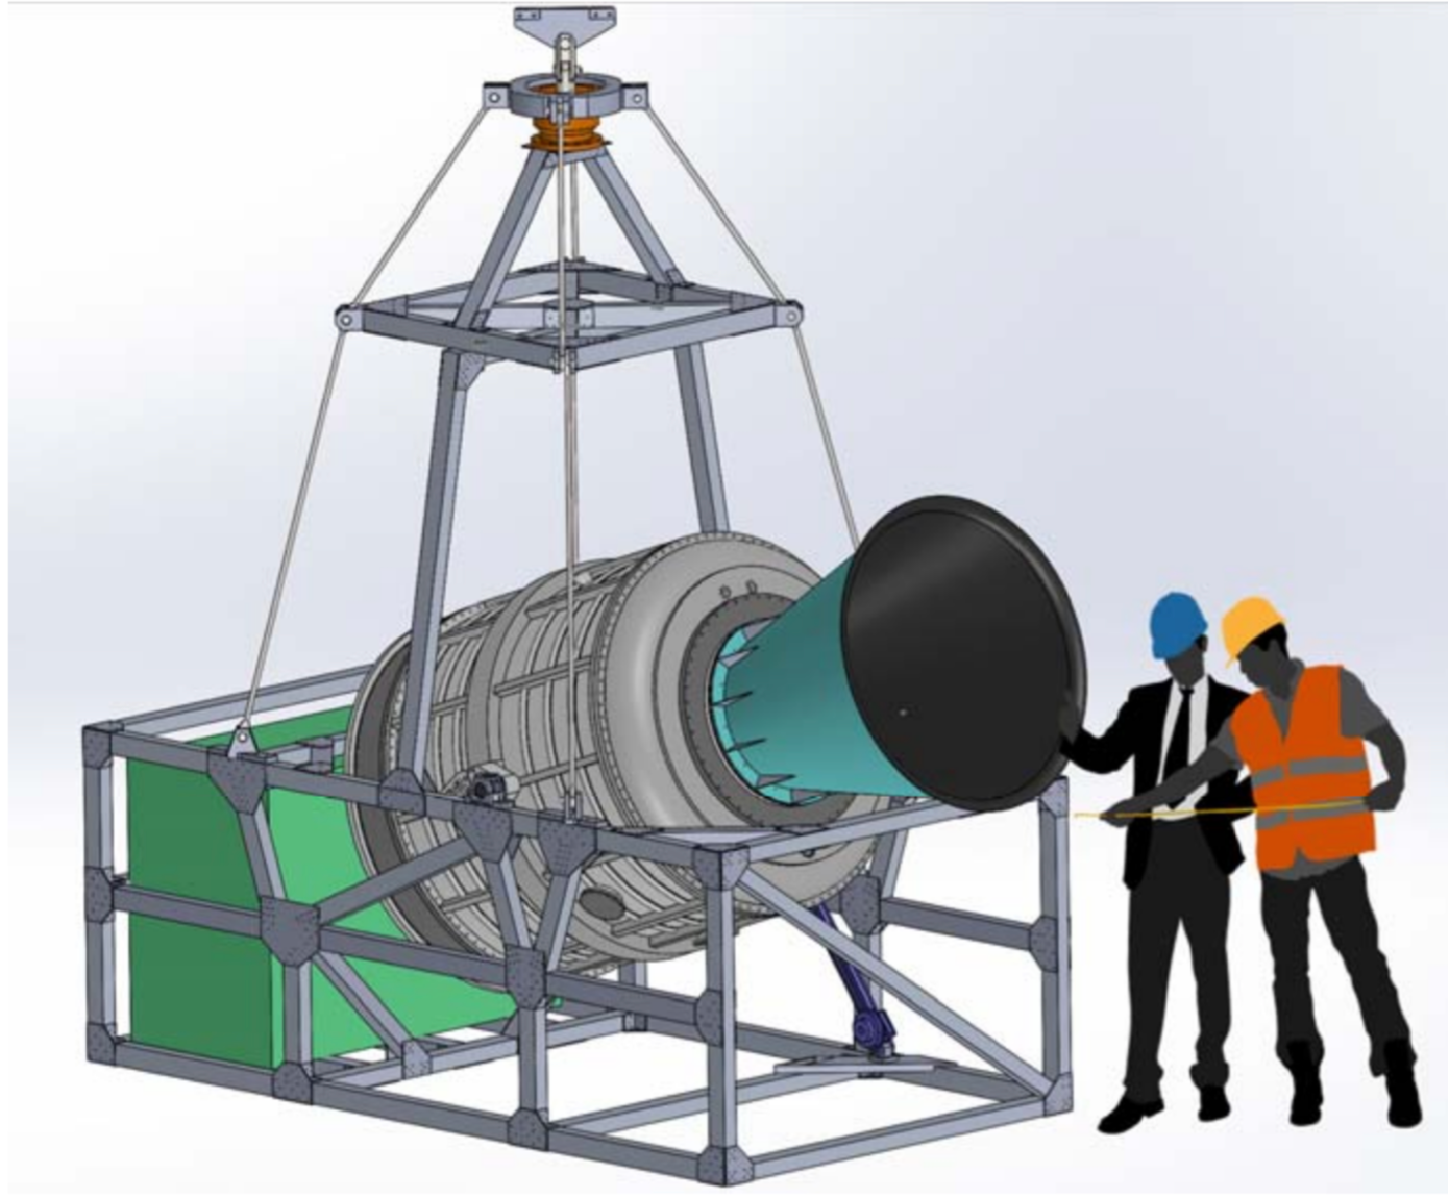
\includegraphics[width=8cm]{figs/swipe_overview.pdf}
   \caption{LSPE-SWIPE overview. The instrument is contained in a large 
   liquid Helium cryostat, which also contains the optical elements, including
   the HWP based Stokes polarimeter. The onboard electronics and the 
   Lithium batteries based power system are contained in an Aerogel 
   insulated box, to optimise thermal balance.  
  }
              \label{fig:swipe_overview}%
    \end{figure}

\subsubsection{Winter polar balloon flight}
\comment{Masi, Piacentini} \\
LSPE-SWIPE is designed to fly on a stratospheric long duration balloon in the arctic winter. 
Ballooning is needed to avoid most of the atmospheric emission, which is very relevant
at 140\,GHz and higher frequencies. The winter launch guarantees the possibility to 
cover a large sky fraction, thus exploring large angular scales of the CMB polarization. 
The instrument is designed to last 15 days. This long duration is needed to reach the
sensitivity to match the scientific goal od LSPE. 

Options for launching in the polar night are ate moment only possible from the 
northern hemisphere. In particular, two proposed launching station is 
Longyearbyen, in Spitsbergen island in Svalbard arcipelago (Norway), with a latitude 
above 78\,$^\circ$N; launches have been organised over the last years from 
this place, both in Summer and in Winter. 
As a more standard alternative, stratospheric balloon flights are organized by the Swedish 
Space Corporation in the Esrange Space Center, near Kiruna (Sweden), at
a latitude of 67.8\,$^\circ$N

Such a long duration flight in the Winter,
without solar illumination, is very demanding in terms of power system, and thermal 
balance. 
A series of technological test flights has been carried out over the years, as
reported in 
\citet{iarocci2008,peterzen_memsait2008,peterzen_cospar2008,peterzen_cospar2010,debernardisIAUS2013,wipica2018}.  
All the LSPE-SWIPE parts are designed to cope with temperatures as low as
$-90^\circ$C, except the battery pack and part of the electronics which is contained in 
a thermally insulated box, designed to work above $-40^\circ$C. This box is insulated
by means of Aerogel. A prototype of this power system was flown in a winter Arctic balloon 
in December 2017 \citep{wipica2018}. 


\subsubsection{Optical system}
\comment{de Bernardis, Lamagna} \\
The optical system of LSPE-SWIPE (Figure~\ref{fig:swipe_optics}) consists in a single-lens, 
490\,mm aperture refractor telescope, focusing incoming radiation 
on two large curved focal planes, split by a large wire-grid polarizer. 
Each focal plane is populated with 165 multi-moded feed-horns, 
each feeding a spider-web Transition Edge Superconducting (TES) 
bolometer. Polarization modulation is obtained rotating a large 
half-wave-plate (HWP) which is the first optical element of the optical 
system.
   \begin{figure}[h!]
   \centering
   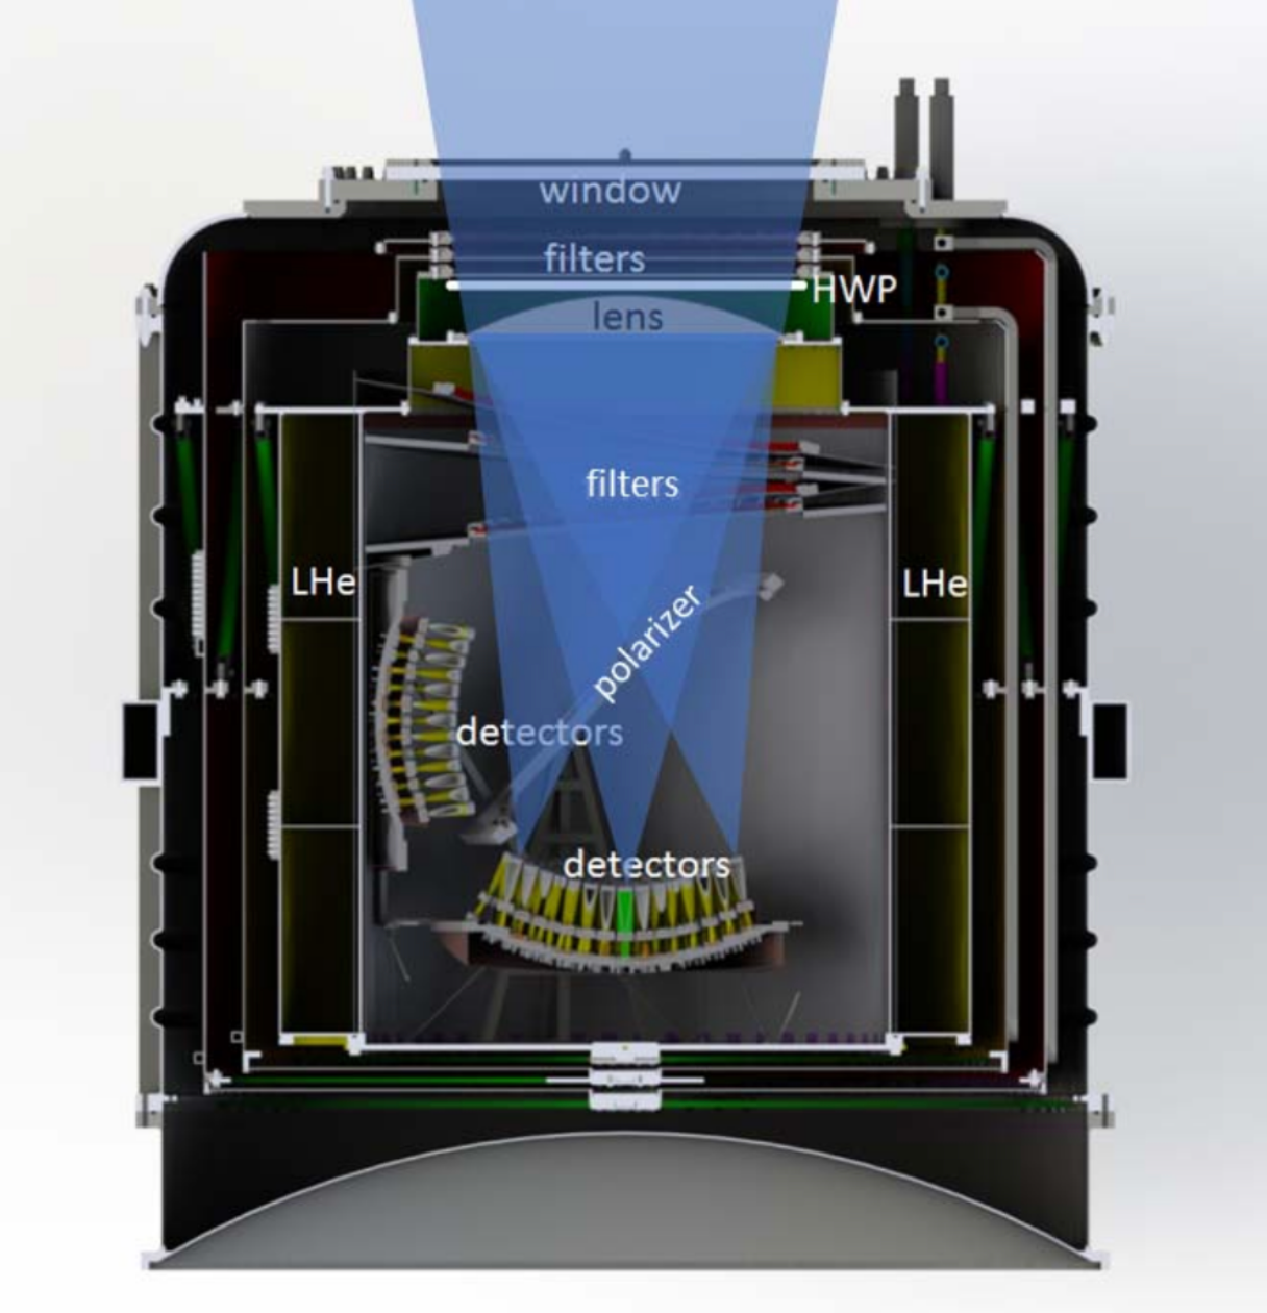
\includegraphics[width=8cm]{figs/swipe_optics_3d}
   \caption{LSPE-SWIPE cryostat and optical optical system
   \comment{Need better figure}}
              \label{fig:swipe_optics}%
    \end{figure}
    
The configuration fulfils our requirements with a low cross-polarization (<0.2\%) 
and a controlled instrumental polarization (an absorption polarization <0.2\% 
and an emitted component reduced and stable by the use of a cold telescope). 
These goals are reached at the edge of the corrected focal plane for all the 3 
bands and they are totally negligible on axis. 
Besides the 490\,mm in diameter lens the optics is completed by a 460\,mm in 
diameter cold stop close to the lens (corresponding to an entrance pupil of 
487\,mm in diameter). 
The FOV, 20\,degrees wide, is split by a 500\,mm in diameter 45\,degress tilted wire grid 
in 2 curved focal plane (CFP\_T and \_R) 300\,mm in diameter both with 
a f/number equal to f/1.75.
The full optical system is kept at cryogenic temperature into the LSPE-SWIPE cryostat, 
in order to minimize radiative background and variable emission from the 
rotating HWP. 

The radiation is coupled to the detectors by means of multimode horns
\citep{legg2016} ....

\comment{Lamagna: add details on horns, in particular mode-coupling}

\subsubsection{Polarization modulation}
\comment{Pisano, Columbro, de Bernardis} \\
In order to modulate the polarized component of the signal, LSPE-SWIPE adopts 
Stokes polarimeter based on a Half Wave Plate (HWP) built of metal mesh 
metamaterials. This technology has been developed by the Instrumentation Group 
at the Department of Physics and Astronomy of the Cardiff University, and 
guarantees homogenous performance over a wide range of frequencies. 

\comment{Pisano: add details about HWP performance}



\subsubsection{Detectors}

\comment{sempre nell'ottica di definire le prestazioni, quindi modi accoppiati, efficienza, 
time constants, e noise}
\\ \comment{Gatti / Lamagna}





\section{Performance forecast, methods}\label{sec:methods}
\subsection{Instrument simulators}
\comment{Piacentini, Tomasi }
Simulators are key elements for instrument design and for data analysis. 
In the design phase, they allow to predict the scientific performance of the 
instruments and the impact of systematic effects. In the data analysis phase, 
they allow to run Montecarlo realizations of the observations, which are 
necessary to estimate instrumental biases, measure transfer functions, 
and to propagate uncertainties. 

The instrument simulator of LSPE-SWIPE consists in a parallel Fortran-90 code
which takes as input:
\begin{itemize} 
\item the number of detectors;
\item the detectors position in the focal plane; 
\item the detectors noise, in terms of NET and 1/f knee frequency;
\item the mission starting date and duration;
\item the angular response in the sky of each detector, as a 2d matrix; this
is convolved in pixel space, in a radius specified also as input parameter;
\item the HWP operation strategy (stepping, spinning, spinning rate, stepping period);
\item the level of HWP synchronous systematic effects, as a signal in $\mu$K$_\text{CMB}$
at the HWP spinning frequency and its harmonics;
\item HWP angle offset or angle statistical uncertainty;
\item timeline filter (high-pass, low-pass or band-pass);
\item map-making algorithm details, as simple re-binning, or iterative
destriping.
\end{itemize}
It generates in output:
\begin{itemize} 
\item timeline of each detector (optional);
\item maps of each detector;
\item map of combined detectors;
\item coverage map;
\item noise covariance 3x3 matrix for each observed pixel.
\end{itemize}

The instrument simulator of LSPE-STRIP is based on ... \comment{Tommasi}


\subsection{Noise estimation}
\comment{de Bernardis for SWIPE, including distribution of detector number in the bands}\\
\comment{Tomasi/Mennella for STRIP}


\subsection{Sky coverage}
\comment{Discuss Swipe/Strip the best observation strategy to maximise overlap.
How low can Strip go in zenithal angle to match Swipe coverage }

\subsection{Component separation}
\comment{Molinari, Pagano, Natoli, Baccigalupi, ...}
Component separation is a mandatory step in the extraction of the CMB polarization 
\citep[see e.g.][]{buzzelli_migliaccio2018}. In particular Galactic Dust and Synchrotron 
emission are the most relevant foreground in polarization. 
In this analysis we consider a template fitting technique, in which the 140 GHz channel
is used to extract CMB polarization, while other channels are used as 
foreground templates to remove foregrounds.
For example, a high frequency channel map, $M_\text{HF}$, can be used 
to trace and remove the dust signal, $M_\text{dust}$, from the 
140\,GHz map, $M_\text{140}$.   
The high frequency map contains dust and CMB signal:
\begin{equation} 
M_\text{HF} = M_\text{CMB} + M_\text{dust}
\end{equation}
while the 140 GHz channel contains CMB and a fraction $\alpha_\text{dust}$ of
the dust in the $M_\text{HF}$ map:
\begin{equation} 
M_\text{140} = M_\text{CMB} + \alpha_\text{dust} \cdot M_\text{dust}
\end{equation}
The CMB map can be extracted as
\begin{equation} 
M_\text{CMB} = \frac{M_\text{140} - \alpha_\text{dust} \cdot M_\text{HF}}{1-\alpha_\text{dust}}
\end{equation}
The noise, $N_\text{CMB}$, in the CMB reconstructed map is then
\begin{equation}
N_\text{CMB}^2 = \left( \frac{1}{1-\alpha_\text{dust}} \right)^2 N_\text{140}^2 + \left( \frac{\alpha_\text{dust}}{1-\alpha_\text{dust}} \right)^2 N_\text{HF}^2
\end{equation}
where $N_\text{140}$ is the noise in the 140\,GHz map, and $N_\text{HF}$ is the noise in the high 
frequency map. 
The coefficient that multiplies the noise in the 140\,GHz map is always larger than 1;
the coefficient that multiplies the noise in the HF map is smaller than 1 if $\alpha_\text{dust} < 0.5$, 
larger otherwise. 
In principle the $\alpha_\text{dust}$ coefficient may be different in different sky patches, but 
we assume a constant value in this analysis. 
\\
\comment{In this paper we mainly focus on noise propagation from template fitting 
technique; an independent paper can describe in detail the template fitting technique}\\
\comment{Include a figure with LSPE frequency bands and spectra of the polarised 
foregrounds } \\
\comment{Dobbiamo decidere come trattare il sincrotrone. In prima approssimazione 
possiamo scrivere che il rumore delle mappe a bassa frequenza, propagato usando 
l'indice spettrale, \`e trascurabile rispetto al rumore della banda a 140 GHz. 
Poi aggiungere un commento su possibile bias dovuto a curvatura dello spettro 
del sincrotrone e spettro non uniforme. In modo da evidenziare l'importanza 
dei canali a bassa frequenza. }

\subsection{Likelihood}
\comment{Pagano/Natoli}

\section{Performance forecast, results}\label{sec:results}

Instrumental configurations: SWIPE flight 8/15 days; SWIPE coverage; STRIP coverage.


See table~\ref{tab:tauerrors} for result on the optical depth $\tau$.\comment{Pagano} 

%
%\begin{table}[htp]
%\begin{center}
%\begin{tabular}{l|c|c|c|c}
%channels & v01 & v02 & v03 &v04 \\
%\hline
%140 & 0.0038 & 0.0043 & 0.0036 & 0.0040\\
%140 c. 220 & 0.0044 & 0.0051 & 0.0042 & 0.0049\\
%140 c. 240 & 0.0049 & 0.0060 & 0.0047 & 0.0056\\
%140 c. 255 & 0.0048 & 0.0056 & 0.0045 & 0.0056\\
%140 c. 270 & 0.0045 & 0.0052 & 0.0043 & 0.0049\\
%140 c. 353 & 0.0042 & 0.0046 & 0.0040 & 0.0043\\
%220 c. 240 & 0.0106 & 0.0138 & 0.0106 & 0.0136\\
%220 c. 255 & 0.0104 & 0.0128 & 0.0097 & 0.0123\\
%220 c. 270 & 0.0096 & 0.0116 & 0.0090 & 0.0116\\
%220 c. 353 & 0.0088 & 0.0102 & 0.0084 & 0.0102\\
%140 c. 353 + 220 c. 270  & 0.0042 & 0.0045 & 0.0039 & 0.0043\\
%140 c. 220 240 353  & 0.0040 & 0.0045 & 0.0038 & 0.0044\\
%140 c. 220 270 353  & 0.0039 & 0.0045 & 0.0039 & 0.0041\\\end{tabular}
%\end{center}
%\caption{$\tau$ 1-$\sigma$ errors obtained marginalizing over $\ln(10^{10}A_{\rm s})$. "c." means "cleaned by".}
%\label{tab:tauerrors}
%\end{table}%


\begin{table}[htp]
\begin{center}
\begin{tabular}{l|c|c}
channels & 8 days & 15 days \\
\hline
140 & 0.0037 & 0.0042\\
140 c. 220 & 0.0048 & 0.0061\\
140 c. 220x2 & 0.0045 & 0.0054\\
140 c. 240 & 0.0053 & 0.0065\\
140 c. 255 & 0.0051 & 0.0059\\
140 c. 270 & 0.0046 & 0.0054\\
140 c. 353 & 0.0041 & 0.0046\\
140 c. 240 + 220 c. 353  & 0.0051 & 0.0061\\
140 c. 255 + 220 c. 353  & 0.0047 & 0.0055\\
140 c. 270 + 220 c. 353  & 0.0046 & 0.0054\\
140 c. 353 + 220 cc. 270  & 0.0041 & 0.0044\\
\end{tabular}
\end{center}
\caption{$\tau$ 1-$\sigma$ errors obtained marginalizing over $\ln(10^{10}A_{\rm s})$. "c." means "cleaned by".
\comment{Scambiare intestazione colonne}}
\label{tab:tauerrors}
\end{table}%

See table~\ref{tab:rerrors} for uncertainty estimation on the tensor to scalar ratio $r$.\comment{Pagano} 

\begin{table}[htp]
\begin{center}
\begin{tabular}{l|c|c}
channels & 8 days & 15 days \\
\hline
140 & 0.011 & 0.019\\
140 c. 220 & 0.036 & 0.059\\
140 c. 220x2 & 0.027 & 0.046\\
140 c. 240 & 0.048 & 0.071\\
140 c. 270 & 0.028 & 0.048\\
140 c. 353 & 0.019 & 0.027\\
140 c. 353 + 220 cc. 270  & 0.019 & 0.027\\
\end{tabular}
\end{center}
\caption{Upper limit at 68\% C.L. on $r$. "c." means "cleaned by". 
\comment{Scambiare intestazione colonne. I valori devono essere aggiornati. }}
\label{tab:rerrors}
\end{table}%

~\\
Spectral index? \comment{possiamo dire qualcosa?} \\ \\
Low-ell anomaly \comment{Gruppuso/Natoli}\\ \\
Birefringence \comment{Melchiorri++} \\ \\
Other science: \\
- non-gaussianity \comment{Matarrese?} , \\
- galactic synchrotron \comment{Nicoletta}, \\
- dust \comment{Masi}



\section{Systematics effects and calibration}\label{sec:systematics}
\comment{Direi che un discorso completo sulle sistematiche richiederebbe un altro articolo. Troppi aspetti da trattare.
Qui ci possiamo limitare a commentare sulle tecniche di mitigazione e di calibrazione che intendiamo utilizzare}

\comment{Piacentini, Natoli, Bersanelli, Tomasi, Columbro, de Gasperis}

\subsection{LSPE-STRIP systematic effects and calibration}
\comment{Bersanelli, Tomasi, Mennella}


\subsection{LSPE-SWIPE systematic effects and calibration}
\comment{de Bernardis, Piacentini, Natoli, de Gasperis, Columbro, Lamagna}

\subsubsection{Instrument requirement}

\comment{From SWIPE Program requirement document. Questa parte pu\`o essere
ridotta, aggiungendo referenze a vari articoli in letteratura, inclusi Buzzelli et al., proceeding 
di Columbro 2018}

LSPE-SWIPE is designed to minimize instrumental polarization. This is the spurious signal resulting
from the measurement of unpolarized radiation. 
In the case of CMB, the amount of unpolarized radiation coming from
the sky is overwhelming with respect to the polarized signal, minimizing instrumental
polarization is the most important driver of instrument design. 
The requirement is that the
maximum acceptable level of instrumental polarization is 0.2\%. 
In this way we will get a constant
polarized signal lower than 6\,mK from the unpolarized background, while from CMB anisotropy we
will get at most 0.2\,$\mu$K spurious polarization, correlated to temperature fluctuations (even less at large
angular scales). The constant signal is treated as an offset in the data analysis, whose stability depends
on the stability of the gain of the electronics and of the responsivity of the detectors, and is not
synchronous with the observed sky. 
Instrumental polarization is reduced during system design using an
optical system close to on-axis, and avoiding mirrors in favor of lenses. The main design choice here
is to have the polarization modulator as the first optical elements in the system, thus relaxing
significantly the requirements on the following optical components.

The second parameter to be considered is cross-polarization. Cross-polarization is defined as the
response of a polarimeter to an input signal polarized in direction orthogonal to the nominal
polarimeter direction. Cross-polarization results in leakage of E-modes into B-modes. 
%Crosspol can be effectively mitigated by means of a precise calibration and data analysis, as confirmed by our
%experience in the data analysis of BOOMERanG and Planck-HFI, where levels of cross-polarization
%around 10% were managed successfully. 
Our requirement is that the maximum acceptable level of cross-polarization is below 2\%. 
This is achieved again by means of an accurate optical design.

The third parameter to be considered is the ellipticity of the main beam (detector angular response 
in the sky). Step rotation or spinning of
the Half Wave Plate allows to observe the same sky region with the same beam orientation, and
different polarimeter orientation. This strongly mitigates the ellipticity requirement, and differential 
ellipticity among different detectors. 
%Previous experience shows that an acceptable level of ellipticity is below 2\%. 
%The main way to achieve this
%is to use an on-axis system and not to use the marginal regions of the focal plane. In our baseline the
%used area of the focal plane is only the central 25\% of the area of the entrance pupil. However, the
%ellipticity in the beam is mainly dictated by the multimode propagation in the horns instead of
%aberration effects along the focal plane. So a smarter optical configuration is under study, which
%should allow to re-gain a larger fraction of the area.

Correct measurement of the angles of the polarimeters is crucial to avoid leakage from E-modes into
B-modes, and to avoid contamination in the measurement of fundamental physics effects such as
cosmic birifringence. In this contest, our system is characterized by the presence of a single, large
wire grid polarizer, defining the reference system for polarization measurements. With this design
the system is similar to an ideal polarimeter, and the angle of the single large wire grid polarimeter
can be accurately measured. We set the requirement for the polarimeter angle measurement to
0.2 degrees. This will improve by at least a factor 10 with respect to e.g. Planck-HFI, where the
polarization axis is defined by the orientation of PSBs, much more difficult to measure due to their
small dimensions \citep{rosset2010}.

Spectral matching among detectors 
has been historically a problem for instruments without a polarization modulator, just comparing
two independent measurements of the orthogonal polarization components. 
In LSPE-SWIPE we use a Stokes polarimeter, where the same detector measures both polarizations,
alternated by means of a rotating half-wave plate. In this configuration the most important requirement is
that the waveplate has high modulation efficiency over the detection bandwidth of the focal plane it
serves. In our system a single waveplate covers all the bands from 120 to 250 GHz. This
requires 70\% bandwidth for the waveplate, a goal certainly reachable with significant
accuracy, by means of metamaterials \citep[see][]{Pisano:06}.
%In addition, band-defining filters and blocking filters should not produce a significant background on
%the detectors and should not allow any leak of high frequency radiation (up to the UV band). We will
%use the same requirements as in the Planck-HFI instrument.

\subsubsection{Half-Wave Plate synchronous effects}
\comment{Columbro }

\citep[see][]{ritacco2017}

\subsubsection{LSPE-SWIPE calibration }
\comment{de Bernardis, Piacentini, Natoli, de Gasperis, Columbro, Lamagna}




\section{Conclusion}\label{sec:conclusion}
\input{conclusion.tex}

 \begin{acknowledgements} 
 LSPE is granted by .... ASI, INFN, ...
\end{acknowledgements}

\bibliographystyle{aa} % style aa.bst
\bibliography{biblio} % your references biblio.bib

\comment{Per i riferimenti bibliografici, input da tutti. Possibilmente bibtex da inserire nel file biblio.bib, oppure DOI, o link ADS}


\end{document}
